\documentclass{beamer}
\usepackage[utf8]{inputenc}
\usepackage[T1]{fontenc}
\usepackage{algorithm}
\usepackage{algpseudocode}
\usepackage{listings}
\usepackage{xcolor}
\usepackage[normalem]{ulem}
\usepackage{tikz-qtree}
\usetikzlibrary{trees}

\definecolor{codegreen}{rgb}{0,0.6,0}
\definecolor{codegray}{rgb}{0.5,0.5,0.5}
\definecolor{codepurple}{rgb}{0.58,0,0.82}
\definecolor{backcolour}{rgb}{0.95,0.95,0.92}

\lstdefinestyle{mystyle}{
   backgroundcolor=\color{backcolour},   
   commentstyle=\color{codegreen},
   keywordstyle=\color{magenta},
   numberstyle=\tiny\color{codegray},
   stringstyle=\color{codepurple},
   basicstyle=\tiny\ttfamily,
   breakatwhitespace=false,         
   breaklines=true,                 
   captionpos=b,                    
   keepspaces=true,                 
   numbers=left,                    
   numbersep=5pt,                  
   showspaces=false,                
   showstringspaces=false,
   showtabs=false,                  
   tabsize=2
}
\lstset{style=mystyle}

\renewcommand{\t}{\text}
\newcommand{\ra}{\longrightarrow}

\usetheme{Boadilla}
\usecolortheme{seahorse}

\title{Korection deux frases incorecte an frases corecte}
\author{Hurot Eliott - 28537} 
\date{2025}
%\logo{\includegraphics[height=1cm]{}}

\begin{document}

\tikzset{
edge from parent fork down,
level distance=1.75cm,
every tree node/.style={align=center}
}

\frame{\titlepage}

\begin{frame}{Problématique}
   \begin{center}
      \huge{Comment peut-on écrire un programme qui corrige des phrases en français ?}
   \end{center}
\end{frame}

\begin{frame}
   \frametitle{Sommaire}
   \tableofcontents
\end{frame}

\section{Objectif}
\begin{frame}
   \frametitle{Objectif du projet}
   \begin{algorithm}[H]
      \caption{Correction de phrases}
      \begin{algorithmic}
         \Require Phrase à corriger - string
         \Ensure Phrase corrigée - string
      \end{algorithmic}
   \end{algorithm}
\end{frame}

\section{Présentation de l'algorithme}
\begin{frame}
   \frametitle{Etapes :}
   \begin{enumerate}
      \item[\Large{1}] \Large{Analyse lexicale (Lexing)}
      \item[2] \Large{Analyse syntaxique (Parsing)}
      \item[3] \Large{Vérification de la phrase}
      \item[4] \Large{Correction de la phrase}
   \end{enumerate}
\end{frame}

\subsection{Stockage des données}
\begin{frame}
   \frametitle{Stockage des données - Trie}
   Structure de donnée qui prend avantage de la similitude entre les clés\\
   \begin{center}
   je - joue - jouer - mire - jouais\\
   \end{center}
   \centering
   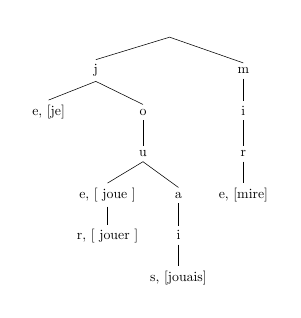
\begin{tikzpicture}[scale=0.5]
   \Tree [.{ }
      [.j 
         [.{e, [je]} ]
         [.o 
            [.u 
               [.{e, [ joue ]}
                  [.{r, [ jouer ]} ] ]
               [.a 
                  [.i 
                     [.{s, [jouais]} ] ] ] ] ] ]
      [.m
         [.i
            [.r
               [.{e, [mire]} ] ] ] ] ]
   \end{tikzpicture}\\
   Taille : 983809 \; \; Hauteur : 39
\end{frame}

\subsection{Analyse lexicale}
\begin{frame}
   \frametitle{Analyse lexicale (Lexing)}
   \begin{algorithm}[H]
      \caption{Analyse lexicale}
      \begin{algorithmic}
         \Require Phrase à corriger - string
         \Ensure Liste de tokens - token list list
      \end{algorithmic}
   \end{algorithm}
   Token : Classe grammaticale, valeur, informations\bigbreak
   Pourquoi token list list ?\\
   Plusieurs sens possibles pour un même mot
\end{frame}

\begin{frame}
   \frametitle{Exemple}
   le petit chat rouge joue\bigbreak
   [[D : le, Ov : le],
    [A : petit, N : petit],
    [N : chat],
    [A : rouge, N : rouge],
    [V : joue, V : joue]]
   \bigbreak
   Complexité ?\\
   O(n * s)\\
   n : nombre de mots dans la phrase\\
   s : taille du mot le plus long de la phrase
\end{frame}

\subsection{Analyse syntaxique}
\begin{frame}
   \frametitle{Analyse syntaxique (Parsing)}
   \begin{algorithm}[H]
      \caption{Analyse syntaxique}
      \begin{algorithmic}
         \Require Liste de tokens - token list list
         \Ensure Arbre syntaxique - syntax\_tree list
      \end{algorithmic}
   \end{algorithm}
   \bigbreak
   LR parser, LL parser
\end{frame}

\subsubsection{Grammaire}
\begin{frame}
   \frametitle{Définition}
   Quadruplet $(V, T, \Sigma, S)$
   \begin{itemize}
      \item $V$ Ensemble de symboles non terminaux
      \item $T$ Ensemble de symboles terminaux
      \item $R$ Ensemble de règles de production de la forme :
                $$X \ra \alpha , ~~ X \in V , ~~ \alpha \in (V \cup T)$$
      \item $S$ Symbole de départ
   \end{itemize}
\end{frame}

\begin{frame}
   \frametitle{Exemple}
   $$3 + 2 + 12$$
   \begin{minipage}{.45\textwidth}
      \begin{tabular}{rcl}
         S & $\longrightarrow$ & N~+~S | N\\
         N & $\longrightarrow$ & [$0$-$9$]~N~|~$\varepsilon$\\
      \end{tabular}
   \end{minipage}
   \hspace{.05\textwidth}
   \begin{minipage}{.45\textwidth}
      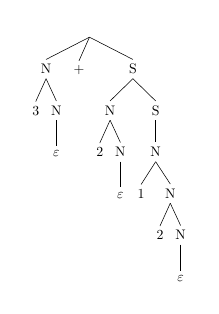
\begin{tikzpicture}[scale = 0.5]
      \Tree [.{}
               [.N
                  [.3 ]
                  [.N 
                     [.{$\varepsilon$} ] ] ]
               [.+ ]
               [.S
                  [.N 
                     [.2 ]
                     [.N 
                        [.{$\varepsilon$} ] ] ]
                  [.S 
                     [.N 
                        [.1 ]
                        [.N 
                           [.2 ]
                           [.N 
                              [.{$\varepsilon$} ] ] ] ] ] ]
      ]
      \end{tikzpicture}
   \end{minipage}
\end{frame}

\begin{frame}
   \frametitle{Grammaire du français (restrictive)}
   \begin{tabular}{lcl|lcl}
      S & $\ra$ & S_u~V_g & V_g & $\ra$ & P~V~C \\
      S_u & $\ra$ & N_g | P_{ps} & P & $\ra$ & Pronom \\
      N_g & $\ra$ & D~A~N~A & V & $\ra$ & verbe | A_V \\
      P_{ps} & $\ra$ & Pronom personnel sujet & A_V & $\ra$ & Auxiliaire~~Verbe \\
      D & $\ra$ & Déterminant & C & $\ra$ & C_{OD} | C_{OI} \\
      A & $\ra$ & Adjectif~A | $\varepsilon$ & C_{OD} & $\ra$ & N_g | V \\
      N & $\ra$ & Nom & C_{OI} & $\ra$ & P_r~N_g \\
      & & & P_r & $\ra$ & Pronom
   \end{tabular}
\end{frame}

\subsection{Vérification \&\& Correction}
\begin{frame}
   \frametitle{Vérification \&\& Correction}
   \begin{algorithm}[H]
      \caption{Vérification \&\& Correction}
      \begin{algorithmic}
         \Require Arbre syntaxique d'un élément - syntax\_tree list
         \Ensure Arbre syntaxique de l'élément corrigé - syntax\_tree list
      \end{algorithmic}
   \end{algorithm}\bigbreak
   2 types d'erreurs : Erreur syntaxique et Fautes de frappe\\
   Exemple : Le petite chat rouge boit du lait\medbreak
   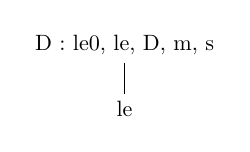
\begin{tikzpicture}[scale=0.8]
   \Tree [.{D : le \\ 0, le, D, m, s}
   [.{le} ] ]
   \end{tikzpicture}
   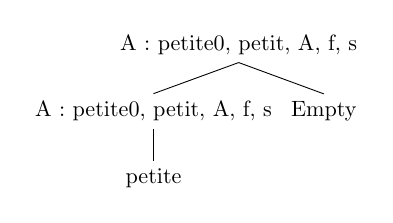
\begin{tikzpicture}[scale=0.8]
   \Tree [.{A : petite \\ 0, petit, A, f, s}
   [.{A : petite \\ 0, petit, A, f, s}
   [.{petite} ] ]
   [.{Empty} ] ]
   \end{tikzpicture}
   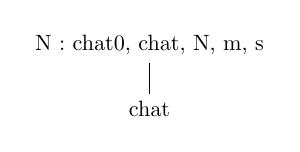
\begin{tikzpicture}[scale=0.8]
   \Tree [.{N : chat \\ 0, chat, N, m, s}
   [.{chat} ] ]
   \end{tikzpicture}
   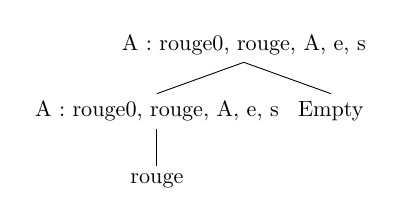
\begin{tikzpicture}[scale=0.8]
   \Tree [.{A : rouge \\ 0, rouge, A, e, s}
   [.{A : rouge \\ 0, rouge, A, e, s}
   [.{rouge} ] ]
   [.{Empty} ] ]
   \end{tikzpicture}
\end{frame}

\begin{frame}
   \frametitle{Vérification \&\& Correction}
   \centering
   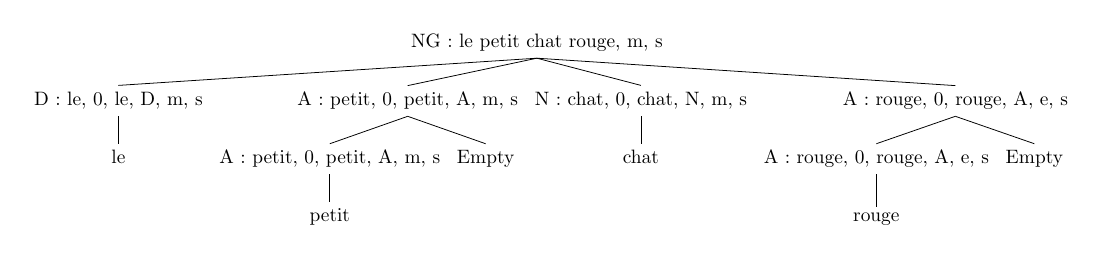
\begin{tikzpicture}[scale = 0.7]  
   \Tree [.{NG : le petit chat rouge \\ , m, s}
      [.{D : le \\ , 0, le, D, m, s}
      [.{le} ] ]
      [.{A : petit \\ , 0, petit, A, m, s}
      [.{A : petit \\ , 0, petit, A, m, s}
      [.{petit} ] ]
      [.{Empty} ] ]
      [.{N : chat \\ , 0, chat, N, m, s}
      [.{chat} ] ]
      [.{A : rouge \\ , 0, rouge, A, e, s}
      [.{A : rouge \\ , 0, rouge, A, e, s}
      [.{rouge} ] ]
      [.{Empty} ] ]
   ]
   \end{tikzpicture}
\end{frame}

\begin{frame}
   \frametitle{Vérification \&\& Correction}
   \centering
   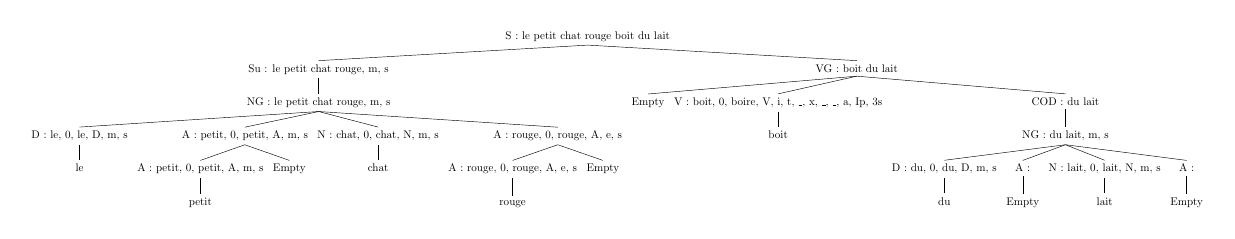
\begin{tikzpicture}[scale = 0.4]
   \Tree [.{S : le petit chat rouge boit du  lait  \\  }
      [.{Su : le petit chat rouge \\ , m, s}
      [.{NG : le petit chat rouge \\ , m, s}
      [.{D : le \\ , 0, le, D, m, s}
      [.{le} ] ]
      [.{A : petit \\ , 0, petit, A, m, s}
      [.{A : petit \\ , 0, petit, A, m, s}
      [.{petit} ] ]
      [.{Empty} ] ]
      [.{N : chat \\ , 0, chat, N, m, s}
      [.{chat} ] ]
      [.{A : rouge \\ , 0, rouge, A, e, s}
      [.{A : rouge \\ , 0, rouge, A, e, s}
      [.{rouge} ] ]
      [.{Empty} ] ]
      ]
      ]
      [.{VG : boit du  lait  \\ }
      [.{Empty} ][.{V : boit \\ , 0, boire, V, i, t, \_, x, \_, \_, a, Ip, 3s}
      [.{boit} ] ]
      [.{COD : du  lait  \\ }
      [.{NG : du  lait  \\ , m, s}
      [.{D : du \\ , 0, du, D, m, s}
      [.{du} ] ]
      [.{A :  \\ }
      [.{Empty} ] ]
      [.{N : lait \\ , 0, lait, N, m, s}
      [.{lait} ] ]
      [.{A :  \\ }
      [.{Empty} ] ]
      ]
      ]
      ]
   ]
   \end{tikzpicture}
\end{frame}

\section{Gestion des résultats}
\begin{frame}
   \frametitle{Gestion des résultats}
   Problème : Trop de corrections possible \\
   Exemple :\\
   la petit chat roug bois du lait $\ra$ 28 corrections possibles\\
\end{frame}

\begin{frame}
   \frametitle{Distance de Levenshtein}
   Distance entre deux chaîne de caractères
   $$
   \t{lev}(a,b) = \begin{cases} \max(|a|,|b|) & \t{si} \min(|a|,|b|) = 0 \\
                                \t{lev}(a-1, b-1) & \t{si} a[0] = b[0] \\
                                1 + \min \begin{cases} \t{lev}(a-1,b) \\ \t{lev}(a, b-1) \\ \t{lev}(a-1, b-1) \end{cases} & \t{sinon}
                  \end{cases}
   $$
   Complexité : O((n+1)*(m+1))\medbreak
   Autre possibilités :\\
   Nombre de correction
\end{frame}

\begin{frame}
   \frametitle{Fréquence d'utilisation}
   Ajout d'une fréquence d'utilisation des mots au dictionnaire\\
   Dictionnaire adapté à l'utilisateur\bigbreak
   Résultats :\medbreak
   Le jeune grçon rames\bigbreak
   \begin{tabular}{ll}
      Distance de levenshtein : &le jeune garçon rame\\
      Fréquence Eschyle : &le jeune garçon ramerait\\
      Fréquence Usuelle : &le jeune garçon rame\\
      Reverso : &le jeune garçon ramène
   \end{tabular}\bigbreak
   Reverso : \guillemotleft Le correcteur français le plus précis au monde \guillemotright
\end{frame}

\begin{frame}
   \frametitle{Fin}
   \centering
   \Huge{\sout{Mairci pour vottre attanssion}}\medbreak
   \Huge{Merci pour votre attention}
\end{frame}

\section{Annexe}

\begin{frame}
   \frametitle{Dictionnaire}
   0,de,de,D,e,i\\
   0,du,du,D,m,s\\
   0,la,le,D,f,s\\
   0,un,un,D,m,s\\
   0,sont,être,V,i,\_,\_,\_,\_,\_,a,Ip,3p\\
   0,être,être,V,i,\_,\_,\_,\_,\_,a,Y\\
   0,ont,avoir,V,i,t,\_,\_,\_,\_,a,Ip,3p\\
   0,été,être,V,i,\_,\_,\_,\_,\_,a,Q,e,i,\\
   0,la,la,N,m,i\\
   0,est,est,N,m,s\\
   0,a,a,N,m,i\\
\end{frame}

\end{document}
